\documentclass[11pt]{article}

\usepackage{amsmath}
\usepackage{graphicx}
\usepackage{subcaption}

\newcommand{\numpy}{{\tt numpy}}    % tt font for numpy

\topmargin -.5in
\textheight 9in
\oddsidemargin -.25in
\evensidemargin -.25in
\textwidth 7in

\begin{document}

% ========== Edit your name here
\author{Aobo Yang (ay6gv)}
\title{CS6316: HW6}
\maketitle

\medskip

% ========== Begin answering questions here
\begin{enumerate}

\item
Unsupervised Learning with Clustering

1.3 K-means Clustering

\medskip

Figure \ref{fig:k_means} is the scatter plot of the K-means.

\begin{figure}[!h]
  \centering
  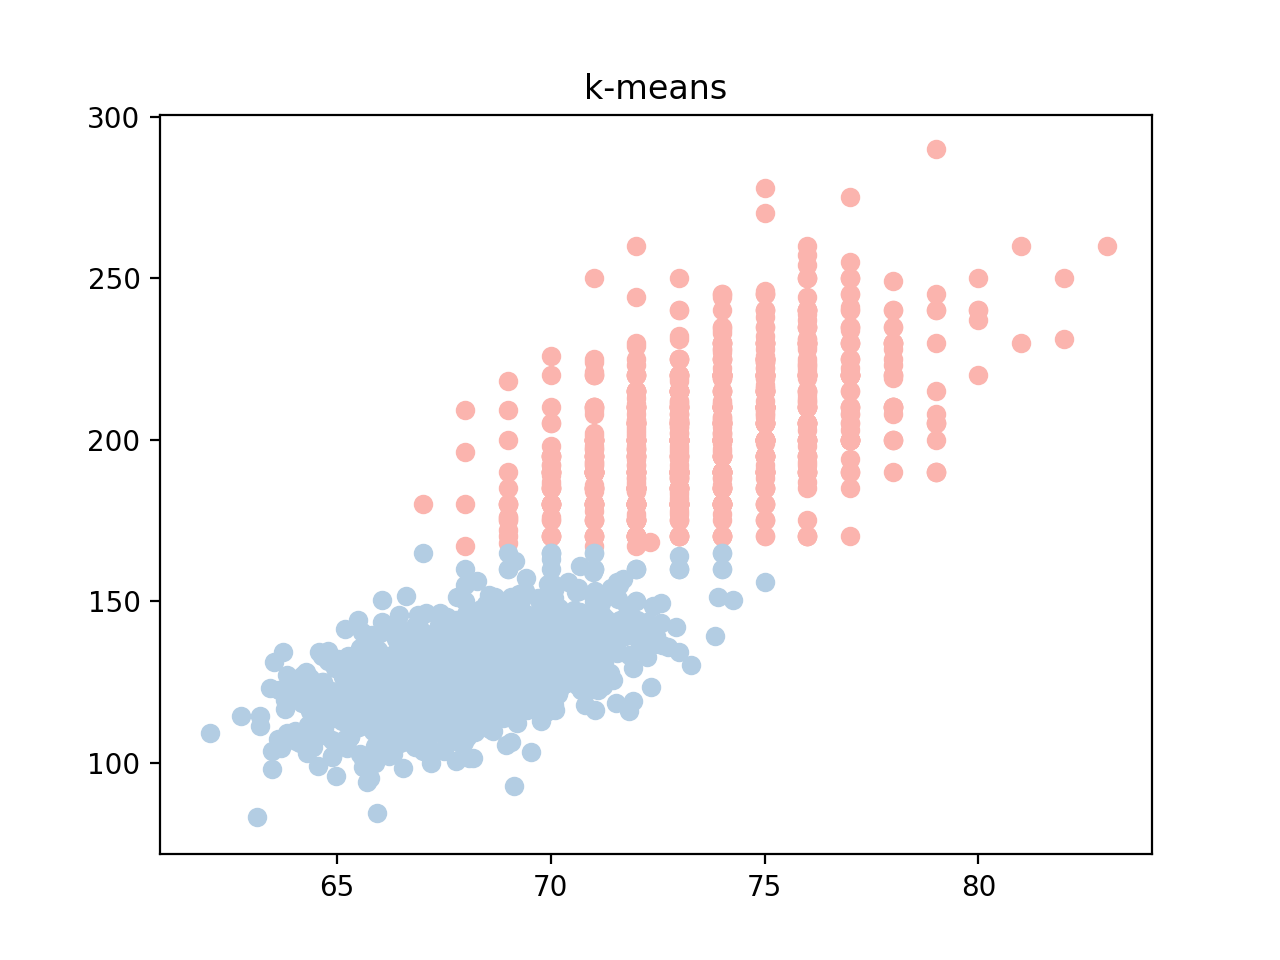
\includegraphics[width=\linewidth]{figures/k_means.png}
  \caption{K-means Scatter Plot}
  \label{fig:k_means}
\end{figure}

The relationship between k and objective function value is shown in Figure \ref{fig:k_knee_finding}.

\begin{figure}[!h]
  \centering
  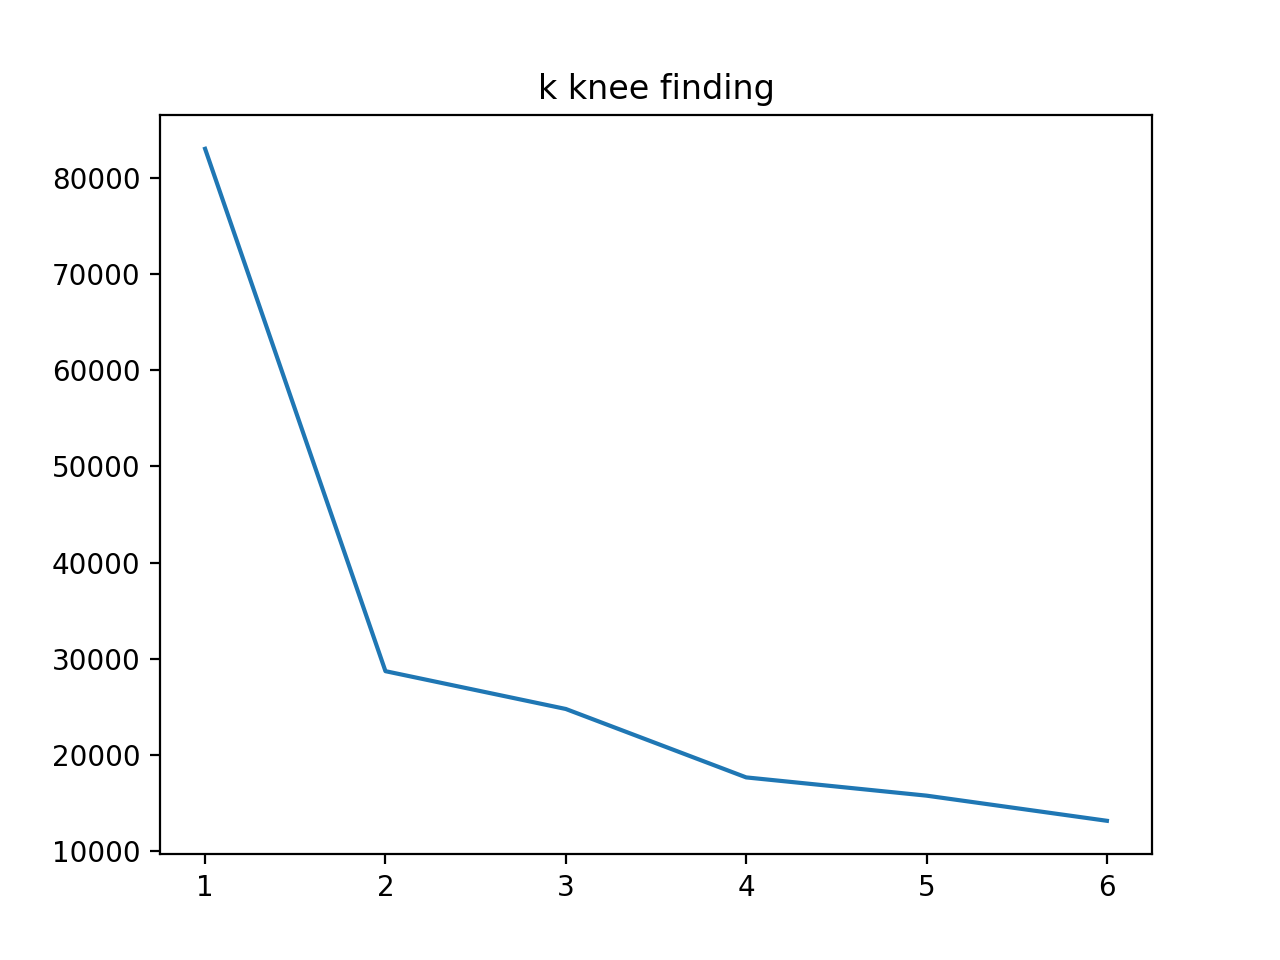
\includegraphics[width=\linewidth]{figures/k_knee_finding.png}
  \caption{K Knee Finding}
  \label{fig:k_knee_finding}
\end{figure}

The purities of clusters when k equals $2$ is shown in the table below

\begin{center}
  \begin{tabular}{ |c|c| }
   \hline
   Cluster & Purity \\
   0 & 0.9990 \\
   1 & 0.9724 \\
   \hline
  \end{tabular}
\end{center}

\medskip

1.4 Guassian Mixture model

Figure \ref{fig:gmm_diag_1} is the scatter plot of the GMM with covType of diag for dataset1.

\begin{figure}[!h]
  \centering
  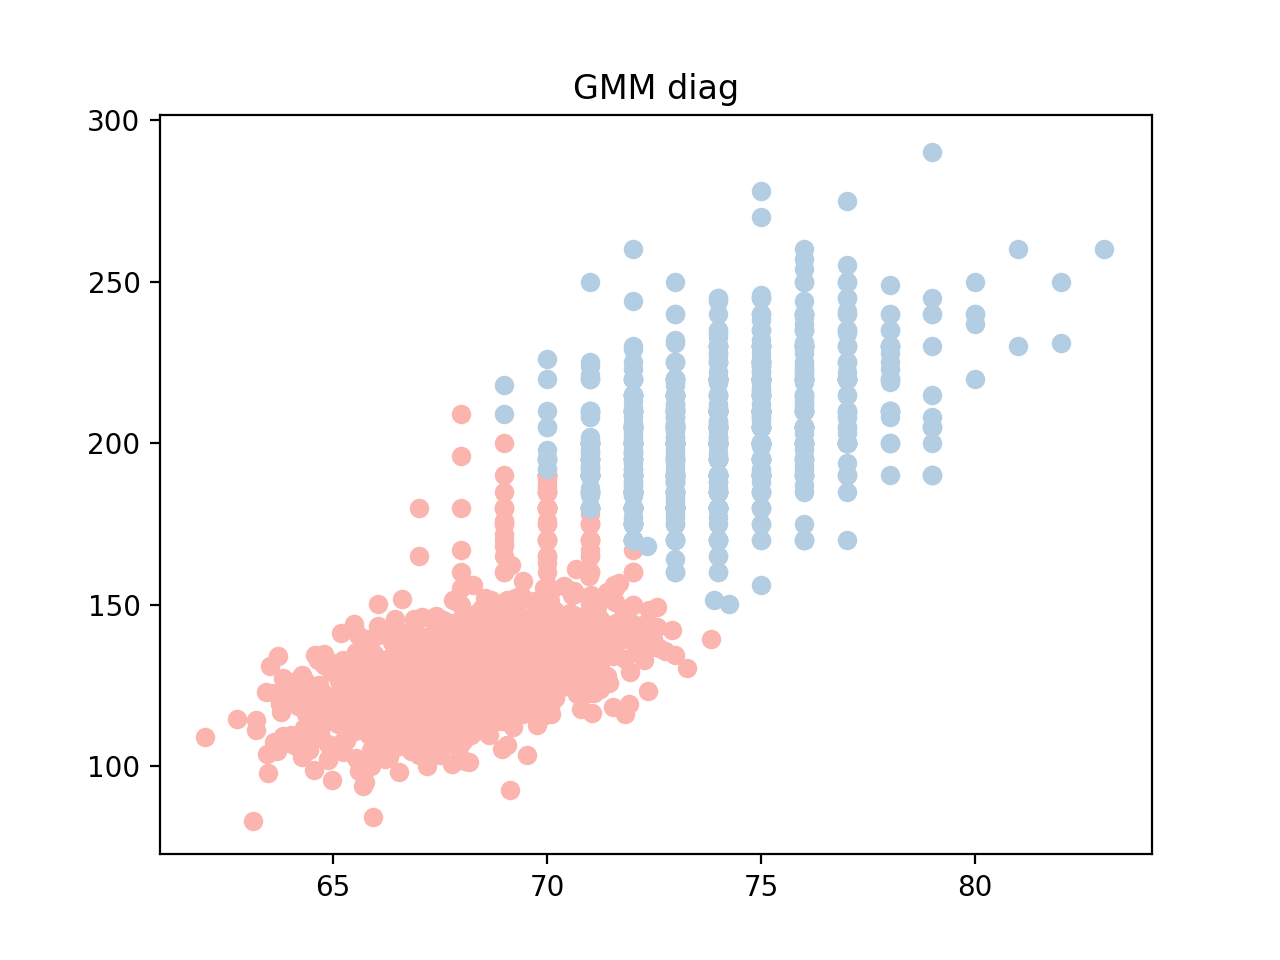
\includegraphics[width=\linewidth]{figures/gmm_diag_1.png}
  \caption{GMM Diag Dataset1 Plot}
  \label{fig:gmm_diag_1}
\end{figure}

Figure \ref{fig:gmm_full_1} is the scatter plot of the GMM with covType of full for dataset1.

\begin{figure}[!h]
  \centering
  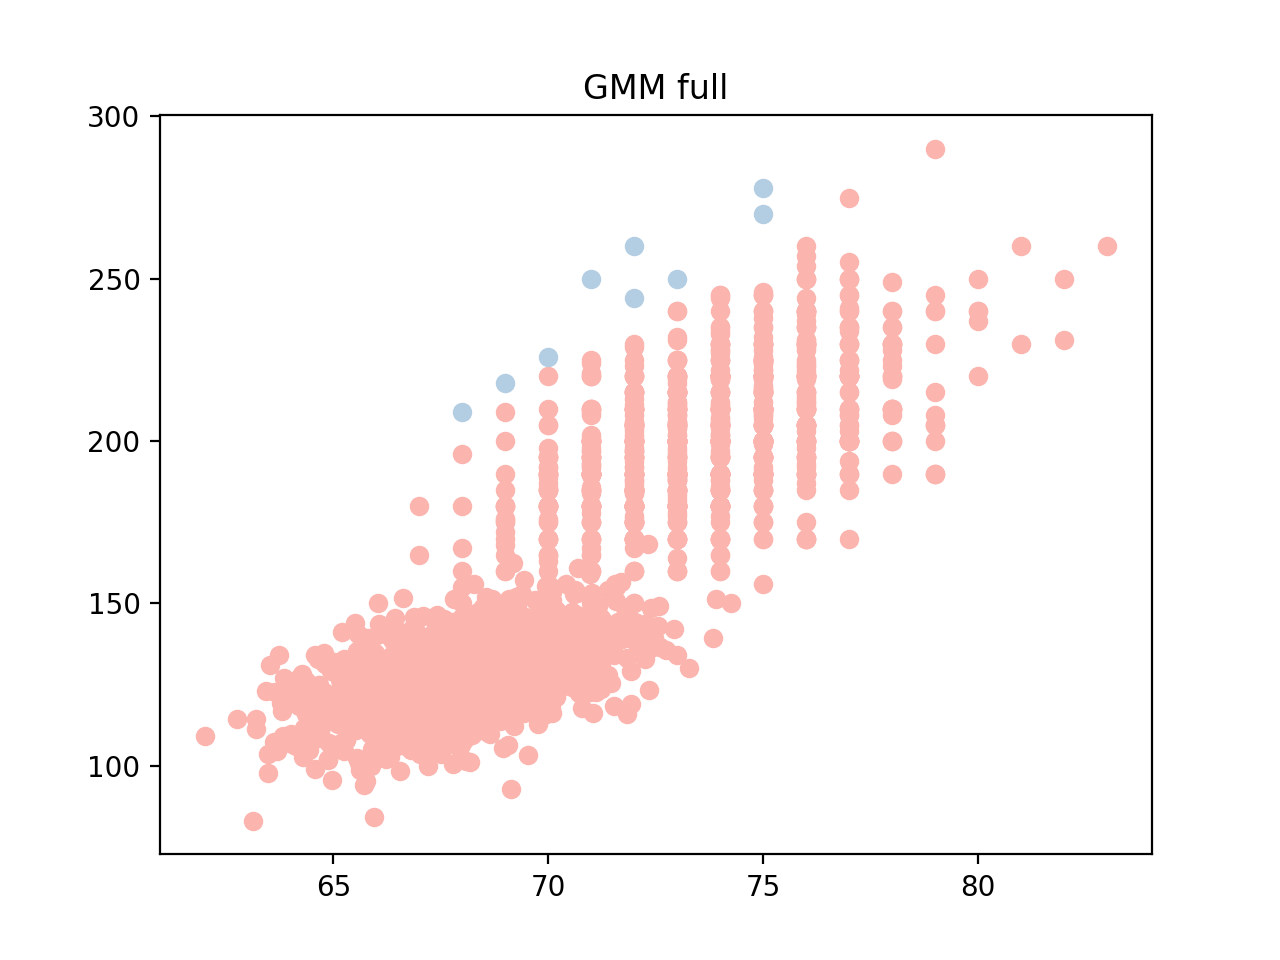
\includegraphics[width=\linewidth]{figures/gmm_full_1.png}
  \caption{GMM Full Dataset1 Plot}
  \label{fig:gmm_full_1}
\end{figure}

Figure \ref{fig:gmm_diag_2} is the scatter plot of the GMM with covType of diag for dataset2.

\begin{figure}[!h]
  \centering
  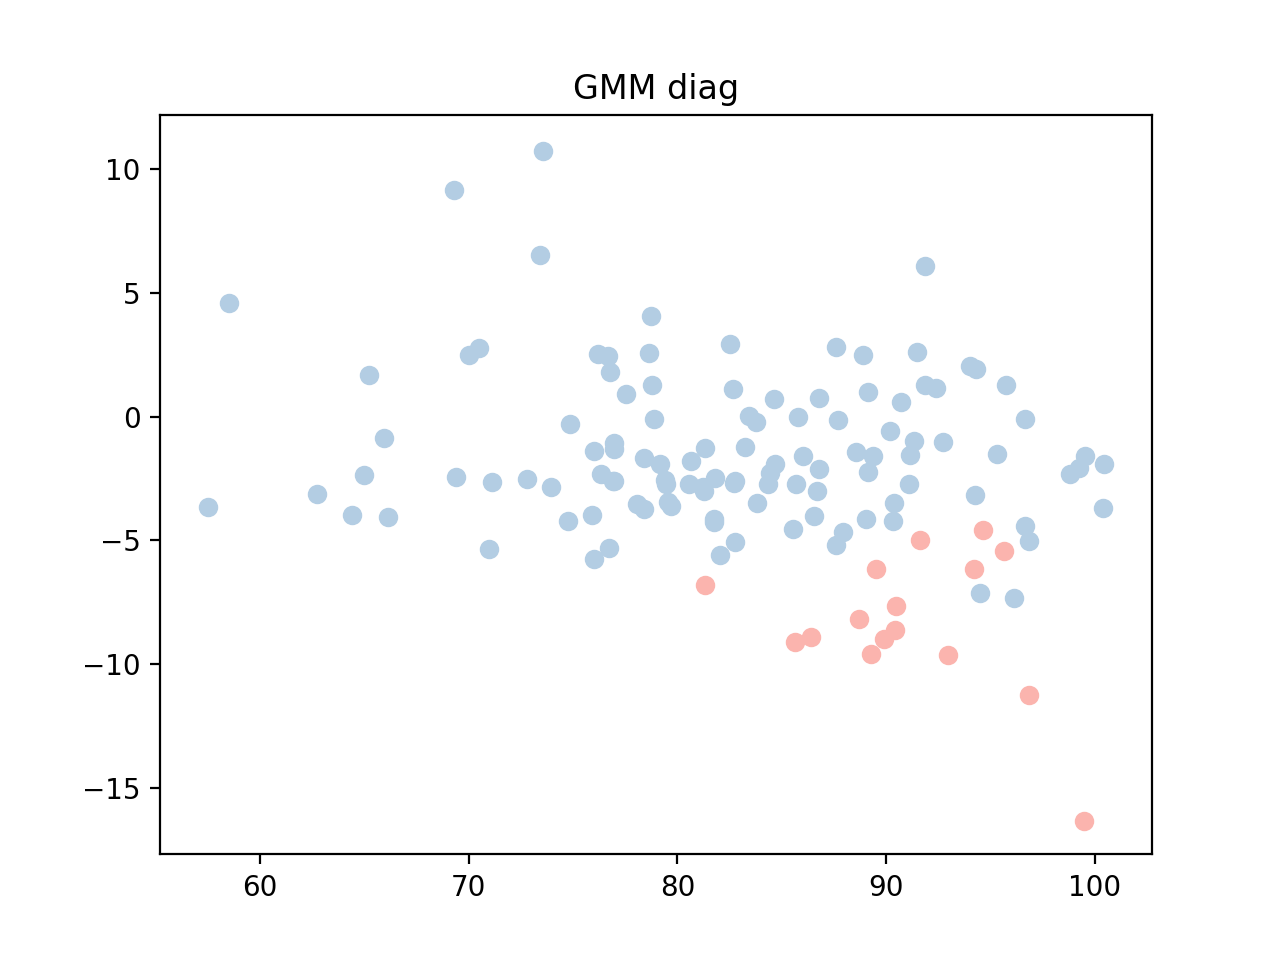
\includegraphics[width=\linewidth]{figures/gmm_diag_2.png}
  \caption{GMM Diag Dataset2 Plot}
  \label{fig:gmm_diag_2}
\end{figure}

Figure \ref{fig:gmm_full_2} is the scatter plot of the GMM with covType of full for dataset2.

\begin{figure}[!h]
  \centering
  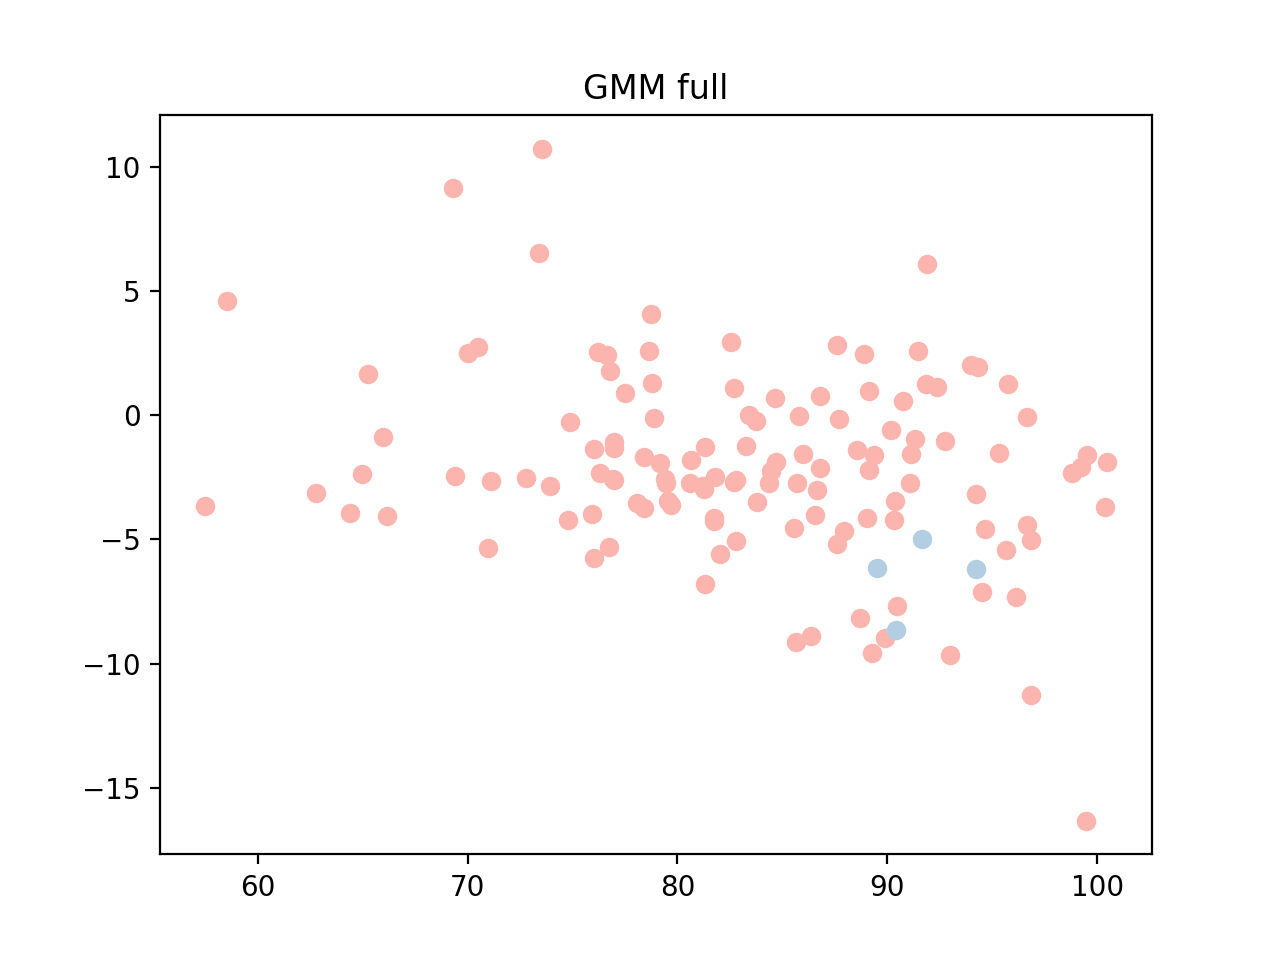
\includegraphics[width=\linewidth]{figures/gmm_full_2.png}
  \caption{GMM Full Dataset2 Plot}
  \label{fig:gmm_full_2}
\end{figure}


The purities of dataset1 with GMM diag are shown in the table below

\begin{center}
  \begin{tabular}{ |c|c| }
   \hline
   Cluster & Purity \\
   0 & 0.9315 \\
   1 & 0.9968 \\
   \hline
  \end{tabular}
\end{center}

The purities of dataset1 with GMM full are shown in the table below

\begin{center}
  \begin{tabular}{ |c|c| }
   \hline
   Cluster & Purity \\
   0 & 1.0 \\
   1 & 0.5394 \\
   \hline
  \end{tabular}
\end{center}

The purities of dataset2 with GMM diag are shown in the table below

\begin{center}
  \begin{tabular}{ |c|c| }
   \hline
   Cluster & Purity \\
   0 & 0.6875 \\
   1 & 0.5268 \\
   \hline
  \end{tabular}
\end{center}

The purities of dataset2 with GMM full are shown in the table below

\begin{center}
  \begin{tabular}{ |c|c| }
   \hline
   Cluster & Purity \\
   0 & 0.5161 \\
   1 & 1.0 \\
   \hline
  \end{tabular}
\end{center}

\item
Sample QA Questions

\medskip

2.1 Bayes Classifier

\medskip

(a)
From the table

$$
P(G=1) = \frac{1}{2} ,\;
P(a=1|G=1) = \frac{1}{2} ,\;
P(b=1|G=1) = \frac{1}{4}
$$

$$
P(G=0) = \frac{1}{2} ,\;
P(a=1|G=0) = \frac{1}{2} ,\;
P(b=1|G=0) = \frac{1}{2}
$$

So

$$
P(a=1 \land b=1 \land G=1) = P(a=1|G=1)P(b=1|G=1)P(G=1) = \frac{1}{16}
$$

$$
P(a=1 \land b=1 \land G=0) = P(a=1|G=1)P(b=1|G=0)P(G=0) = \frac{1}{8}
$$

$$
P(a=1 \land b=1) = P(a=1 \land b=1 \land G=1) + P(a=1 \land b=1 \land G=0) = \frac{3}{16}
$$

$$
P(G=1|a=1 \land b=1) = \frac{P(a=1 \land b=1 \land G=1)}{P(a=1 \land b=1)} = \frac{1}{3}
$$

\medskip

(b)

False, NB is a generative model which gets $p(C|X)$ indirectly through modeling $p(C)$ and $p(X|C)$ while logistic regression is a discriminative model which indeed models $p(C|X)$

\medskip

(c)

False, they assume each feature $p(X_j|cluster==i)$ follows Gaussian distribution not the whole data point $X$.

\medskip

(d)

False, because Gaussian Naive Bayes classifier is a special case of QDA that the covariances are all diagonal matrices, but as long as the covariances are different, the decision boundary is quadratic as QDA.

% ========== Continue adding items as needed

\end{enumerate}

\end{document}
\grid
\grid
